\section{Načítání dat}

\subsection{Načítání knihovny LDraw}
Mechanizmus načítání a aktualizace knihovny LDraw je implementován s~využitím Symfony komponenty Console. Administrátor aplikace může spouštět jednotilvé příkazy podle instrukcí uvedených v~dodatku \ref{append:instalace}. Na základě těchto příkazů jsou následně načítána data do databáze a prováděn převod formátu. V~ukázce kódu \ref{ukazka-prikaz-ldraw} je možné vidět volání příkazu pro načtení knihovny LDraw.

\begin{listing}[htbp]
        \begin{minted}{bash}
$ bin/console app:load:ldraw --all
------------------------------------------------------------------------
Downloading LDraw library
------------------------------------------------------------------------
Loading file from: http://www.ldraw.org/library/updates/complete.zip
[33.93 MB / 33.93 MB] [===========================]  100% (1 min/1 min)
LDraw libary downloaded
------------------------------------------------------------------------
Loading models from LDraw library: /tmp/printabrick.HIH6lN/ldraw/
------------------------------------------------------------------------
[9782 / 9782] [===========================] 100% (6 mins/6 mins) 
Done with "0" errors.
        \end{minted}
    \caption{Ukázka příkazu pro načtení knihovny LDraw\label{ukazka-prikaz-ldraw}}
\end{listing}

Aplikace umožňuje načítání a aktualizaci celé knihoviny i jednotlivých součástek. Proces načítání jednotlivé součástky je znázorněn na diagramu \ref{schema-nacitani} a podrobněji popsán v~následujících podsekcích.

\begin{figure}[htbp]
    \centering
    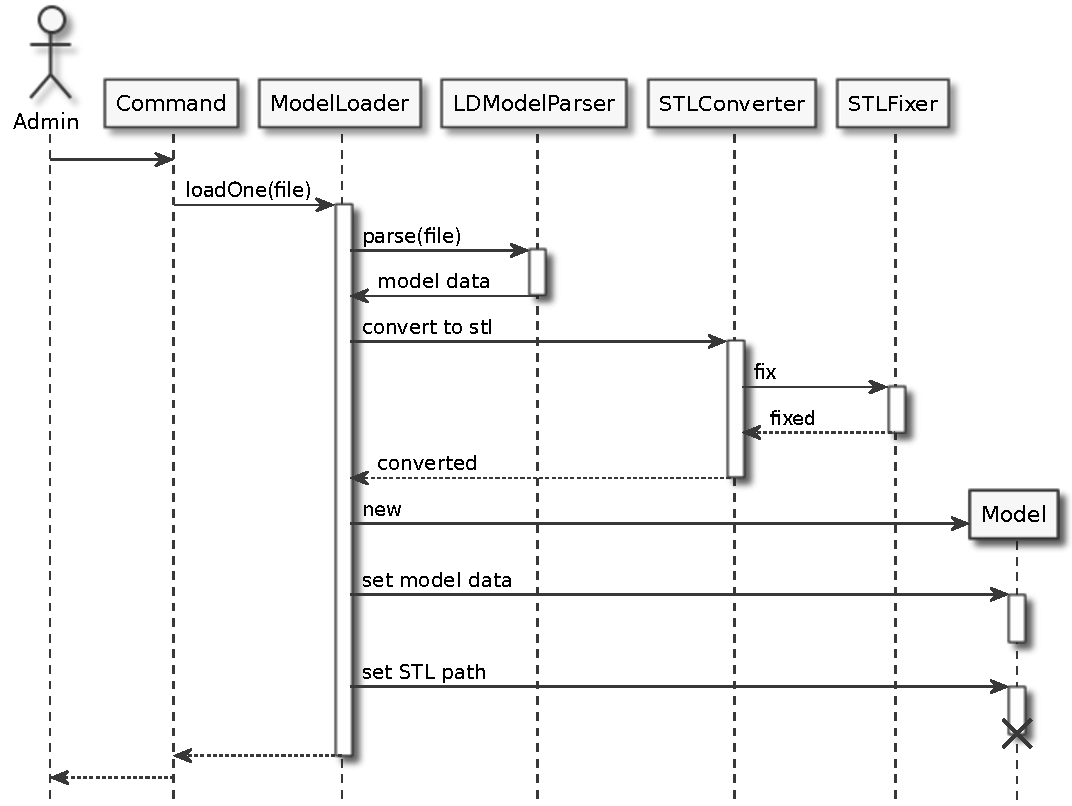
\includegraphics[width=\textwidth,height=\textheight,keepaspectratio]{pdfs/loading.pdf}
    \caption{Diagram načítání součástky knihovny LDraw \label{schema-nacitani}}
\end{figure}

\subsubsection*{Parsování součástek LDraw}
Parsování součástek formátu LDraw má na starost třída \textit{LDModelParser}. Třída na základě specifikace formátu LDraw představeného v~sekci \ref{ldraw-format} parsuje hlavičku souboru i reference na podsoučástky. Data jsou následně v~podobě asociativního pole vrácena k~dalšímu zpracování.

\subsubsection*{Převod formátu}
Pro spouštění programů zajišťující převod formátu LDraw na formát \textit{\gls{STL}} jsem využil komponenty Symfony Process \autocite{symfony:process}. Ta umožňuje spouštění příkazů přímo z~kódu PHP (ukázka kódu \ref{ukazka-stlconverter}).

Převod formátu je nejprve zajištěn třídou \textit{STLConverter}, která zastřešuje volání programu LDView (představeného v~sekci \ref{podsekce-ldview}). Následně třída \textit{STLFixer} provede opravu \textit{\gls{STL}} souboru pomocí volání programu ADMesh (představeného v~sekci \ref{podsekce-admesh}).


\begin{listing}[htbp]
        \begin{minted}{php}
/**
 * Call LDView process with $arguments.
 *
 * @param array $arguments
 */
private function runLDView(array $arguments)
{
    $builder = new ProcessBuilder();
    $process = $builder
        ->setPrefix($this->ldview)
        ->setArguments($arguments)
        ->getProcess();

    $process->run();

    if (!$process->isSuccessful()) {
        throw new ProcessFailedException($process);
    }
}
        \end{minted}
    \caption{Ukázka použití komponenty Symfony Process \label{ukazka-stlconverter}}
\end{listing}

\subsubsection*{Logování}
Protože během procesu načítání knihovny dochází ke zpracování velkého množství dat a ne vždy se dá spoléhat na validitu vstupu, bylo třeba implementovat mechanizmus logování událostí. Významné události a chyby jsou logovány pomocí knihovny Monolog \autocite{symfony:monolog}. Ukázka přidávání události do logu je možné vidět v~ukázce kódu \ref{ukazka-log-udalost} a podobu souboru logu v~ukázce kódu \ref{ukazka-log}.

\begin{listing}[htbp]
        \begin{minted}{php}
try {
    $modelArray = $this->ldModelParser->parse(file_get_contents($file));
} catch (ParseErrorException $e) {
    $this->logger->error($e->getMessage(), [$file]);

    return null;
} catch (FileException $e) {
    $this->logger->error($e->getMessage(), [$file]);

    return null;
}
        \end{minted}
    \caption{Ukázka použití knihovny Monolog \label{ukazka-log-udalost}}
\end{listing}

\begin{listing}[htbp]
        \begin{minted}{text}
[2017-05-27 22:54:05] loader.INFO: Model skipped. {"number":"004695a","type":"Sticker"} []
[2017-05-27 22:54:05] loader.INFO: Model skipped. {"number":"004695b","type":"Sticker"} []
[2017-05-27 22:54:05] event.ERROR: Subpart file not found {"subpart":"2-4cyli","model":"3820"} []
        \end{minted}
    \caption{Ukázka logu načítání\label{ukazka-log}}
\end{listing}

\subsection{Načítání dat Rebrickable}\label{nacitani-rebrickable}
Načítání velkého množství dat z~CSV souborů do aplikace může být dle \autocite{grok} velmi problematické. Načítání databáze Rebrickable má na starost služba \textit{RebrickableLoader}. Ta pomocí volání MySQL funkce \mintinline{text}{LOAD DATA LOCAL INFILE} (viz ukázka kódu \ref{ukazka-nacitani-csv}) načítá velmi rychle CSV soubory Rebrickable.

\begin{listing}[htbp]
        \begin{minted}{php}
private function loadCsvFile($file, $table, $columns)
{
    $query = sprintf("LOAD DATA LOCAL INFILE '%s' 
        REPLACE INTO TABLE %s
        CHARACTER SET UTF8
        FIELDS TERMINATED BY ',' OPTIONALLY ENCLOSED BY '\"'
        LINES TERMINATED BY '\\n'
        IGNORE 1 LINES %s", addslashes($file), $table, $columns);

    return $this->em->getConnection()->prepare($query)->execute();
}
        \end{minted}
    \caption{Ukázka načítání tabulek CSV \label{ukazka-nacitani-csv}}
\end{listing}

\subsection{Mapování LDraw a Rebrickable}
Jedním z~problémů, který vyvstává při využití různých zdrojů dat pro obdržení 3D modelů součástek a databáze stavebnic je vzájemné namapování těchto dat. Namapování součástek má na starost třída \textit{RelationMapper}, která provádí přiřazení součástek z~knihovny LDraw k~součástkám z~databáze Rebrickable. 

Protože obě služby používají lehce odlišný systém číslování součástek (i přes fakt, že číslování Rebrickable vychází z~LDraw), nelze při zohlednění všech pravidel LDraw \autocite{ldraw:numbering:faq} i Rebrickable \autocite{rebrickable:numbering:changes} automaticky rozpoznat vazby všech součástek.

K~umožnění manuálního přiřazení modelů a spoučástek jsem implementoval mechanizmus umožňující definování vazeb pomocí \gls{YAML} souboru \textit{app/Resources/relations/part\_model.yml}. K~načtení souboru je využita komponenta Symfony Yaml Component \autocite{symfony:yaml}. Ukázka mapování součástky na model je možné vidět v~ukázce kódu \ref{ukazka-parovani}. Tyto vazby jsou následně zohledněny při běhu příkazu pro spárování modelů a součástek.

\begin{listing}[htbp]
        \begin{minted} {yaml}
#rebrickable_part_ID: ldraw_model_ID
970d00: 970c00
298c04: 4592c01
        \end{minted}
    \caption{Ukázka part\_model.yml \label{ukazka-parovani}}
\end{listing}

\subsection{API Brickset}
Dalším zdrojem dat využívaným pro obdržení informací o~stavebnicích je API Brickset. Jak již bylo zmíněno v~sekci \ref{reserse-brickset}, API Bricsket je implementováno jako služba postavená nad protokolem \gls{SOAP}. V~PHP je pro komunikaci se SOAP servery k~dispozici třída \textit{SOAPClient} \autocite{soapclient}, která za nás obstarává komunikaci na základě definice v~podobě \gls{WSDL} souboru. 

Při získávání statických dat přes API je vhodné využít možnosti cachování k~minimalizaci počtu dotazů na server a k~urychlení načítání dat. K~tomuto jsem využil komponenty DoctrineCacheBundle. V~ukázce kódu \ref{ukazka-cache} je zobrazena metoda \mintinline{php}{getSetInstructions} třídy \textit{BricksetManager}, která načítá insturkce k~postavení stavebnice z~cache (pokus se zde data již vyskytují) nebo pomocí Brickset API. 

\begin{listing}[htbp]
        \begin{minted} {php}
public function getSetInstructions($id)
{
    $key = 'instructions-'.$id;

    if (!$data = unserialize($this->cache->fetch($key))) {
        $data = $this->bricksetClient->getInstructions($id);
        $this->cache->save($key, serialize($data), self::CACHE_LIFETIME);
    }

    return $data;
}
        \end{minted}
    \caption{Ukázka načtení instrukcí stavebnice\label{ukazka-cache}}
\end{listing}